\documentclass[a4paper,twoside]{article}
\usepackage{listings}
\usepackage{xcolor}
\usepackage{changepage}
\usepackage{graphicx}
\usepackage[hungarian]{babel}
\usepackage{amsmath} 
\usepackage{t1enc}
\usepackage{titlesec}
\title{Szakdolgozat}

\definecolor{mygreen}{RGB}{0,128,0}
\definecolor{mygray}{RGB}{204,255,153}
\definecolor{mymauve}{RGB}{204,102,0}
\definecolor{myblue}{RGB}{0,0,204}
\definecolor{mypurple}{RGB}{204,0,204}

\graphicspath{{./images}}
\author{Bozsik József}

\lstdefinestyle{javascriptStyle}{
	language=Python,  % Change this to JavaScript
	basicstyle=\ttfamily,  % Keyword style for the second keyword list
	commentstyle=\color{mygreen},
	stringstyle=\color{mymauve},
	numberstyle=\tiny\color{mygray},
	numbers=left,
	stepnumber=1,
	numbersep=10pt,
	backgroundcolor=\color{white},
	frame=single,
	rulecolor=\color{black},
	showspaces=false,
	showstringspaces=false,
	showtabs=false,
	tabsize=2,
	captionpos=b,
	frame=none,
	breaklines=true,
	morekeywords=[1]{let, const, async, var, function, return, else, for, while},
	keywordstyle=[1]\color{myblue}, % Use keywordstyle1 for the first set of keywords
	morekeywords=[2]{if,await,},
	keywordstyle=[2]\color{mypurple}, % Use keywordstyle2 for the second set of keywords  % Add 'await' to the morekeywords list
	escapeinside={(*@}{@*)},
	xleftmargin=0pt,
	xrightmargin=0pt,
}

\begin{document}
\maketitle
\newpage
\tableofcontents
\newpage
{\centering
\section*{Hallgatói nyilatkozat}}
Alulírott \textit{Bozsik József}, szigorló hallgató kijelentem, hogy ezt a szakdolgozatot meg
nem engedett segítség nélkül, saját magam készítettem, csak a megadott forrásokat (szakirodalom, eszközök stb.) használtam fel. Minden olyan részt, melyet szó szerint, vagy
azonos értelemben, de átfogalmazva más forrásból átvettem, egyértelműen, a forrás megadásával megjelöltem.
Hozzájárulok, hogy a jelen munkám alapadatait (szerző(k), cím, angol és magyar
nyelvű tartalmi kivonat, készítés éve, konzulens(ek) neve) a BME VIK nyilvánosan hozzáférhető elektronikus formában, a munka teljes szövegét pedig az egyetem belső hálózatán
keresztül (vagy autentikált felhasználók számára) közzétegye. Kijelentem, hogy a benyújtott munka és annak elektronikus verziója megegyezik. Dékáni engedéllyel titkosított diplomatervek esetén a dolgozat szövege csak 3 év eltelte után válik hozzáférhetővé.
\begin{flushleft}
	Budapest, 2022. december 6.
\end{flushleft}

\newpage
\section{Összefoglaló}
A szakdolgozat témájaként egy társasjáték készítését választottam webes környezetben mivel személy szerint mindig is érdekelt a teljes web-fejlesztési folyamat, valamint egyik kedvenc időtöltéseim közé tartozik a barátokkal egy közös társasjátékozás. 
Végül egy ''ki nevet a végén'' társas fejlesztése mellett döntöttem, hiszen a szabályok nem túl bonyolultak, viszont sok lehetőség van kreatívnak lenni az implementálás során, valamint inspirálódni is lehet az eddig elkészült játékokból amik az interneten megtalálhatók.

Társasjáték lévén, a játékot több felhasználó is játszhatja egyszerre.  Az interneten rengeteg olyan web-alkalmazás van, ahol hasonló társasjátékkal
lehet játszani, viszont a belépés nehézkes, a játék kezelése bonyolult. A célom az volt, hogy
egy letisztult felületen könnyedén és egyszerűen lehessen élvezni a társasjáték adta
élvezeteket a partnereinkkel.

Ebben a dokumentumban összefoglalom, hogy hogyan implementáltam, mind a szerveroldali,
mind a kliensoldali szoftvert. Az alkalmazás készítése során rengeteg újfajta technológiát és
keretrendszert használtam, amik jól bevált eszközök a webfejlesztésben. A munkahelyem
által biztosított szervert is használtam a megvalósításához, ami a játék logikáját biztosította. A
végeredmény egy egyszerű, és könnyen kezelhető webalkalmazás lett, ami kis
továbbfejlesztéssel versenytársa lehet az interneten található játékoknak.


\newpage
\section{Abstract}
As the topic of my thesis, I chose to create a board game in a web environment. Personally, I've always been interested in the entire web development process, and one of my favorite pastimes is playing board games with friends. Ultimately, I decided to develop a "Who Laughs Last" board game because the rules are not overly complicated, offering ample room for creativity during implementation, as well as inspiration from existing online games.

Given that it's a board game, multiple users can play it simultaneously. While there are many web applications offering similar board games online, the entry process can be cumbersome, and game management can be complex. My goal was to provide a clean interface for easily enjoying the board game with partners.

In this document, I summarize how I implemented both the server-side and client-side software. Throughout the application development, I utilized various new technologies and frameworks, proven tools in web development. I also used a server provided by my workplace to support the game's logic. The end result is a simple and user-friendly web application that, with some further development, could become a competitor to existing online games.
\newpage
\section{Bevezetés}
A webfejlesztés a mindennapi internetes böngészés során használt weboldalak és
webalkalmazások létrehozásának folyamata. Amikor egy weboldalt látogatunk, például
közösségi média platformokat, online vásárlási oldalakat vagy hírportálokat, akkor a
webfejlesztés végtermékét látjuk.
A weboldalakat programozási nyelvek, keretrendszerek és eszközök kombinációjával építik
fel. A webfejlesztés két fő komponense a frontend és a backend.
A frontend az, amit egy weboldalon látunk és amivel interakcióba lépünk. Ide tartozik az
oldal tervezése, elrendezése és felhasználói felülete, valamint a felhasználói inputok
ellenőrzése is. A frontend létrehozásához a fejlesztők olyan nyelveket használnak, mint az
HTML\footnote{Hypertext Markup Language}, CSS\footnote{Cascading Style Sheets} és a JavaScript. Az
HTML strukturálja a weboldal tartalmát, a CSS pedig esztétikus megjelenést biztosít, míg a
JavaScript interaktivitást és funkcionalitást ad hozzá.
A backend felelős a weboldal háttérlogikájáért és feldolgozásáért. Feladatokat lát el, mint az
adatok tárolása és lekérdezése, felhasználói azonosítás és a szerverkommunikáció. A
fejlesztők különböző programozási nyelveket és keretrendszereket, például az én esetemben
Java Spring\cite{javaspring}-re esett a választás mivel a munkahelyemen ezt a környezetet használják a
backend létrehozásához. Emellett adatbázisokkal kommunikálnak az információ tárolásához
és lekérdezéséhez. Az én implementációmban az utóbbi nem történt meg, hiszen a
munkahelyem által biztosított szerveren tároltam az adatokat.
A webfejlesztés gyakran API\footnote{Application Programming Interface} hívásokat tartalmaz más
szerverek felé adatok lekéréséhez vagy specifikus műveletek végrehajtásához. Ezek az API
hívások lehetővé teszik a különböző rendszerek közötti kommunikációt és információcsere
zavartalan működését. Közismert hasonlat az API-ra, hogyha egy étteremben a konyha
részleg a backend, az asztalok a frontend, ahol a vendégek (felhasználók) ülnek, akkor az API
a pincér, aki kézbesíti az ételt (adatokat).
A következő fejezetekben ismertetem, hogy az alábbi technológiákat miként valósítottam
meg, és milyen keretrendszereket használtam, amik a fejlesztést, és a felhasználói élményt is
egyaránt segítik.
\newpage
\section{Használt technológiák}
A modern webfejlesztésben szinte elengedhetetlen különböző keretrendszerek használata,
mivel a hatékonyságban, és a szoftverminőségben is jelentősen tud segíteni a fejlesztő
számára.
\subsection{Vue.js}
Munkhelyi környezetben a Vue.js\cite{vuejs} keretrendszert használtuk. A Vue.js egyszerűséget,
reaktivitást és komponens alapú architektúrát hangsúlyozva lehetővé teszi a \mbox{fejlesztők}
számára az interaktív és dinamikus webalkalmazások könnyű létrehozását.\\

\textit{\Large{Fő jellemzői: }}
\begin{itemize}
	\item \textbf{Deklaratív megjelenítés: }A Vue.js a Vue sablonok nevű deklaratív szintaxist
	használja, amely lehetővé teszi a fejlesztők számára, hogy HTML-szerű kóddal
	határozzák meg a felhasználói felület szerkezetét és megjelenését. A keretrendszer
	automatikusan frissíti a megjelenített eredményt, amikor az adatok megváltoznak,
	biztosítva a reaktív felhasználói felületet
	\item \textbf{Komponens alapú architektúra: }A Vue.js támogatja az újrafelhasználható és
	moduláris komponensek használatát. A komponensek tartalmazzák mind az UI\footnote{User Interface}-t, mind az azzal kapcsolatos viselkedést, ami átláthatóbbá és skálázhatóbbá
	teszi a kódbázist. A komponensek egymásba ágyazhatók, összeilleszthetők és
	újrahasználhatók az alkalmazás teljes területén.
	\item \textbf{Vue direktívák: }A Vue.js számos direktívát biztosít, amelyek lehetővé teszik a
	fejlesztők számára a dinamikus viselkedés hozzáadását a DOM-hoz (Document Object
	Model). A direktívák, például a v-if, v-for és v-bind, lehetővé teszik a fejlesztők
	számára az elemek feltételes megjelenítését, a lista iterálását és az adatkötést HTML
	attribútumokhoz vagy stílusokhoz.
	\item \textbf{Reaktív adatkötés: }A Vue.js reaktív adatrendszert használ. Amikor az adatok
	megváltoznak, a keretrendszer automatikusan frissíti a megfelelő UI komponenseket,
	biztosítva az adatmodell és a nézet szinkronizációját. Ez könnyűvé teszi a reaktív és
	interaktív felületek létrehozását
	\item \textbf{VueRouter: }A Vue.js rendelkezik egy hivatalos útválasztó könyvtárral, amit Vue
	Routernek hívnak, és amely lehetővé teszi a navigációt. Lehetővé teszi, hogy
	dinamikusan töltsünk be komponenseket, amik gyakran URL változásokkal járnak
\end{itemize}

\subsection{Pinia Store}
Továbbá elterjedt megoldás állapotkezelő mintát alkalmazunk a frontend megvalósítása
során. Erre a Pinia Store\cite{pinia}-t könyvtárat használtam, ami reaktív és hatékony módon
biztosít egy centralizált tárolót az alkalmazás állapotának kezelésére.
\\

A Pinia segítségével definiálhatunk tárolókat, amelyek tárolják az alkalmazásod állapotát,
és különböző metódusokat határozhat meg az állapot módosításár. Minden tároló külön
példányként jön létre, lehetővé téve az alkalmazás állapotának területenkénti vagy funkció
szerinti elválasztását és \mbox{szervezését}.
\\

A Pinia egyik fő előnye a reaktivitási rendszere. A Vue reaktivitását használja fel, hogy
automatikusan frissítse a komponenseket, amikor az állapot a tárolóban megváltozik. Ez
biztosítja, hogy az alkalmazásod mindig szinkronban legyen, és lehetővé teszi a
felhasználói felület hatékonyabb megjelenítését.
\subsection{Webpack}
A Webpack\cite{webpack} egy népszerű modulbundler JavaScript alkalmazásokhoz. Gyakran
használják webfejlesztésben ahhoz, hogy egy alkalmazás különböző moduljait,
erőforrásait és függőségeit egyetlen fájlba vagy fájlcsoportba csomagolja. A Webpack fő
célja a teljesítmény optimalizálása és a modern webalkalmazások bonyolultságának
kezelése.
\\

A Webpack moduláris megközelítést alkalmaz, amely lehetővé teszi a fejlesztők számára,
hogy a kódbázist külön modulokra bontsák. Elemzi ezeknek a moduloknak a függőségeit
és létrehoz egy függőségi gráfot. Ezen gráf alapján a Webpack összecsomagolja a
modulokat, feloldja a függőségeket és generálja a végső kimeneti fájlokat.
\subsection{Axios}
Az Axios\cite{axios} egy JavaScript könyvtár, amelyet a böngészőkben és a Node.js környezetben
is használnak aszinkron HTTP kérések küldésére és fogadására. Az Axios könnyű
használatú, egyszerű szintaxissal rendelkezik, és számos előnyös funkciót nyújt a hálózati
kommunikációhoz.

\textit{\large{Fő előnyök: }}
\begin{itemize}
	\item \textbf{Kényelmes API kezelés: }Az Axios egyszerű és jól strukturált API-t biztosít a
	HTTP kérések kezeléséhez. Különböző HTTP metódusokat, például GET, POST,
	PUT, DELETE stb. használhatunk a kérések elküldésére.
	\item \textbf{Aszinkron működés: } Az Axios aszinkron kérések kezelésére épül, amely
	lehetővé teszi az alkalmazás folyamatosságát és reaktivitását. Nem blokkolja a fő
	szálat, így más műveletek végrehajtására is lehetőséget ad.
\end{itemize}
\begin{adjustwidth}{0cm}{0cm}
	\begin{minipage}{\textwidth}
		\begin{lstlisting}[style=javascriptStyle,caption={HTTP kérés Axios könyvtárral}]
		async function robotStep() {
			
			const boardStore = useBoardStore();
			const gamePlayStore = useGamePlayStore();
			await new Promise(resolve => setTimeout(resolve, 600));
			if (gamePlayStore.playingBoard.status !== 'FINISHED' && gamePlayStore.robotEnabled && boardStore.joinedPlayer.some(p => p.id === gamePlayStore.currentPlayer.id)) {
				await gamePlayStore.rollDice(boardStore.startedBoard.id, { playerId: gamePlayStore.currentPlayer.id });
				await gamePlayStore.movePlayer(boardStore.startedBoard.id, { pieceId: gamePlayStore.selectedPiece?.id, playerId: gamePlayStore.currentPlayer.id, token: gamePlayStore.rollResponse.token });
			}
		}
		\end{lstlisting}
	\end{minipage}
\end{adjustwidth}

 

\subsection{JavaSpring}
A backend részt JavaSpringben\cite{javaspring} valósítottam meg. A Spring lehetővé teszi a gyors és hatékony
webalkalmazások építését, miközben egy rugalmas és moduláris környezetet biztosít a
fejlesztőknek.
\begin{itemize}
	\item  \textbf{Inversion of Control - IoC:} A Spring keretrendszer alapvetően az IoC elvet követi,
	amelyben a keretrendszer vállalja a felelősséget az objektumok létrehozásáért,
	konfigurálásáért és összekapcsolásáért. Ez lehetővé teszi a komponensek laza
	összekapcsolását és könnyen cserélhetővé teszi az implementációkat.
	\item \textbf{Dependency Injection - DI:} A Spring keretrendszer segítségével a dependency
	injection könnyen megvalósítható. Ez azt jelenti, hogy a szükséges objektumokat egy
	külső forrásból szúrhatjuk be a komponensekbe anélkül, hogy a komponenseknek
	maguknak kellene létrehozniuk vagy tudniuk kellene róluk. Ez elősegíti a lazán
	összekapcsolt és könnyen karbantartható kód írását.
	\item \textbf{Webalkalmazás támogatás:} A Spring keretrendszer számos modult és komponenst
	kínál a webalkalmazások fejlesztéséhez. A Spring MVC (Model-View-Controller)
	modell segítségével könnyedén készíthetünk hatékony és rugalmas webes
	alkalmazásokat. A Spring Boot pedig egy továbbfejlesztett modul, amely lehetővé
	teszi a gyors és egyszerű konfigurációt és a gyors indítást.Több előnye is van a Spring
	keretrendszernek, viszont mivel az alkalmazásom bonyolultsága nem követelte meg a
	használatukat, így ezeket nem részletezném.
\end{itemize}

\subsection{Lombok}
A Lombok\cite{lombok}  egy Java nyelvű könyvtár, amely
segít csökkenteni a boilerplate kódot és növeli a fejlesztési produktivitást. A boilerplate kód olyan alapvető vagy sablonkód, amely gyakran
ismétlődő és rutinszerű feladatokra szolgál. A Lombok annotációkat használva lehetővé teszi, hogy a fejlesztők egyszerűbben és gyorsabban hozzanak létre Java osztályokat. Annotációkat a programozásban gyakran használnak, mivel segítik a kód megértését, segíthetik a fejlesztőt a kódírás minimalizálásában, vagy akár a
dokumentáció írásában. A Java nyelvben többféle annotációk léteznek. Ilyenek például a beépített annotációk, amik segítik a kód
megértését. A @Deprecated annotációval ellátott elemeket jelölik, hogy elavultak vagy nem ajánlottak használatra. Ez figyelmezteti a fejlesztőket, hogy más megoldást vagy alternatívát kell használni.

\subsection{Keycloak}
Az autentikációhoz a Keycloak\cite{keycloak} nyílt forráskódú keretrendszert választottam. A Keycloak egy sor olyan funkciót kínál, amelyek segítenek az alkalmazások és szolgáltatások biztonságosításában, ideértve a Single Sign-On (SSO), felhasználói hitelesítést, felhasználói engedélyezéseket és az azonosítás közvetítését. A Single Sign-On (SSO) egy olyan hitelesítési és azonosítási technológia, amely lehetővé teszi a felhasználók számára, hogy egyszeri bejelentkezéssel hozzáférjenek több különböző alkalmazáshoz vagy rendszerhez anélkül, hogy minden egyes alkalmazásban külön-külön be kellene jelentkezniük. Ennek előnyei közé tartozik a a felhasználói kényelem, szigorú ellenőrzés, könnyebb felhasználói ellenőrzés. A Keycloak olyan megoldást nyújt, amely egyszerűsíti a biztonság hozzáadásának folyamatát az alkalmazásokhoz, és lehetővé teszi a felhasználói azonosításokat, szerepeket és jogosultságokat központilag történő kezelését. A keretrendszer képes integrálódni különböző alkalmazásokkal és platformokkal, így értékes eszköz azoknak a szervezeteknek, akik webalkalmazásaikat és API-ikat szeretnék biztonságossá tenni.Támogat különböző hitelesítési módszereket, beleértve a közösségi bejelentkezéseket, több tényezős hitelesítést és még sok mást. Emellett a Keycloak rendkívül rugalmas és bővíthető architektúrával rendelkezik, így alkalmas különféle felhasználási esetekre, a kis alkalmazásoktól a nagyvállalati rendszerekig. Gazdag API-kat kínál, és egy felhasználóbarát adminisztrációs konzolt, amely segít a felhasználók, valóságok és ügyfelek kezelésében.


\subsection{Konva}
A játék megjelenítéséhez a Konva\cite{konva} könyvtárat haszáltam. Konva egy HTML5 Canvas alapú grafikus könyvtár, amelyet használhatunk a webes alkalmazásokban és weboldalakon történő rajzoláshoz és grafikai elemek kezeléséhez. Ez a könyvtár lehetővé teszi a fejlesztők számára, hogy könnyedén rajzolhassanak formákat, vonalakat, szövegeket és egyéb grafikai elemeket a webes felületeken, és interaktív alkalmazásokat hozzanak létre, ahol a felhasználók rajzolhatnak, mozgathatnak és manipulálhatnak grafikai elemeket.Az alábbiakban néhány kulcsfontosságú tulajdonság és funkció, amelyeket a Konva nyújt:

\begin{itemize}
	\item \textbf{HTML5 Canvas alapú:} Konva a HTML5 Canvas API-t használja, ami lehetővé teszi a közvetlen grafikus rajzolást a webes felületeken. Ez rendkívül hatékony és lehetővé teszi a komplex grafikai elemek létrehozását.
	\item \textbf{Interaktivitás:} Konva lehetővé teszi az interaktív grafikus elemek létrehozását, például húzható és áthelyezhető elemeket, melyekre kattintva változtathatjuk az állapotukat.
	\item \textbf{Rétegek és Csoportok:} A könyvtár támogatja a rajzok elrendezéséhez használt rétegek és csoportok létrehozását, ami rendszerezheti és kezelheti a grafikai elemeket.
	\item \textbf{Szöveg és betűtípusok:} Konva lehetővé teszi a szöveges elemek létrehozását, és támogatja a különböző betűtípusok és formázási lehetőségek használatát.
	\item \textbf{Animáció:} A könyvtár animációt támogat, így a grafikai elemek mozgathatók és animálhatók.
	\item \textbf{Eseménykezelés:} Konva lehetővé teszi az események kezelését, például kattintásokat és húzásokat, ami lehetővé teszi az interaktív műveletek megvalósítását.
	\item \textbf{Több platform támogatása:} A Konva nem csak böngészőkben használható, hanem akár Node.js környezetben is, ami különféle alkalmazások fejlesztését teszi lehetővé.
\end{itemize}


\subsection{Postman}
A backend API teszteléséhez, frontend nélkül, kiváló megoldást kínál a Postman\cite{postman}, így ezt használtam a fejlesztés során.Az alábbiakban néhány kulcsfontosságú jellemzőt és funkciót ismertetek, amit a Postman kínál:

\begin{itemize}
	\item \textbf{API Tesztelés:} Postman segítségével könnyedén készíthetsz és futtathatsz API-teszteket. Különböző HTTP kéréseket küldhetsz az API-hoz, és az eredményeket vizsgálhatod.
	\item \textbf{Környezetek és Változók:} Lehetőséged van környezeteket és változókat definiálni a kérésekben, ami lehetővé teszi különböző környezetek (pl. fejlesztési, tesztelési, élő) közötti könnyű váltást és paraméterezést.
	\item \textbf{Automatizálás:} Postman segítségével automatizálhatod az API-teszteket és kéréseket. Például létrehozhatsz kollekciókat, amelyeket később futtatni tudsz automatizált módon.
	\item \textbf{Hitelesítés és Biztonság:} A Postman lehetővé teszi különböző hitelesítési mechanizmusok, például API kulcsok vagy OAuth használatát. Emellett támogatja a biztonsági teszteket is.
\end{itemize}




\newpage

\section{Feladatkiírás pontosítása és részletes elemzése}
Magát a feladatot a külső konzulensem adta meg és specifikálta, hogy mire kell, hogy képes
legyen az alkalmazás, valamint milyen technológiákat használjunk. Maga az implementációt
teljesen rám bízta, hogy milyen osztályokat valósítok meg, azokat hogyan csoportosítom és
hogy hogyan dolgoznak együtt.
A ki nevet a végén társas szabályai vannak érvényben. Tehát egy játékos bábuja csak akkor
tud belépni a táblára, ha 6-ost dob. Ha viszont 6-ost dob valaki, akkor utána még egyszer
dobhat. Ha egy bábu ugyan arra a mezőre lép, ahol már éppen áll egy bábu, akkor leüti a
pályáról. Az a játékos győz, aki leghamarabb, az összes bábuját körbeviszi a táblán.
Mivel a web alkalmazást egy munkahelyi környezetben valósítottam meg, ott már adva volt
egy szerver, ami lényegében egy adatbázis-szerverként funkcionált, valamint játék bizonyos
szintű logikája is már implementálva volt. Tehát az alkalmazás backendjének kommunikálnia
kellett ezzel a szerverrel és feldolgoznia a válaszokat. Erre RESTful API-ra kellett küldeni a
kéréseket. RESTful API egy architekturális stílus és koncepció, amely a webes szolgáltatások
tervezését és fejlesztését írja le. A REST\footnote{Representational State Transfer} alapelveit követve
a RESTful API egy szabványos módszert nyújt a kommunikációra kliensek és szerverek
között. Ezeket az adatokat felhasználva a backend tovább küldi a frontendnek, ahol ezeket
megjeleníti.
Az alkalmazás főoldalán megjelennek az eddig létrehozott táblák, valamint információk
ezekről (hány játékos lépett már be, mennyi a maximum létszám, elindult-e már a játék,
stb…). 

Egyszerre akár több játékost is beállíthatunk. Ezután elindítjuk a pályát, ami átnavigál egy
újabb oldalra, ahol a tábla van megjelenítve. Egy adott táblának 3 státusza lehet: CREATED,
STOPPED, FINISHED. A CREATED státuszban A kockadobás egy sima gomb, amit ha a
felhasználó megnyom, generál egy számot 1-től 6-ig. Ezután rákattint a bábura amit mozgatni
szeretne, és az a megfelelő mennyiséggel előre lép a táblán. Ha éppen ellenfél játékosra lép,
leüti a tábláról. Ha az összes bábu beér akkor kiírja, hogy nyert az adott játékos és maga a
tábla átvált FINISHED státuszra. 
\newpage

\section{Önálló munka bemutatása}
Első részben az alkalmazás backendjét írtam meg, valamint mert felépítésben is így tűnt
logikusnak. Az osztályokat rétegekbe rendeztem funkciójuk és függőségeik szerint.
\subsection{Backend}
A Model rétegbe tettem azokat az osztályokat, amiket majd, később a hálózaton elküldök egy
http (HyperText Transfer Protocol) kérésbe ágyazva a szervernek, majd a válaszokat is ezekbe
az osztályokba konvertálom át. Az egész backenden ezekkel az objektumokkal dolgozok.
A DAL (Data Acces Layer)-be tettem azokat az osztályokat amik kommunikálnak a
szerverrel. Esetünkben a nevezéktan egy kicsit megtévesztő, hiszen hagyományos web
alkalmazás esetén ez a réteg az adatbázissal kommunikál, ám ennek hiányában nekünk erre
nincs lehetőségünk. Az elnevezést viszont megtartottam, hiszen gondolhatunk a szerverünkre,
mint egy okos adatbázisra, ami ismeri a ki nevet a végén társas szabályait, valamint, ha egy
másik fejlesztő olvasná a kódomat, egyből tudná, hogy az adott rétegnek mi a felelőssége.
Ezekben az osztályokban indítom el a http kéréseket, valamint a válaszokat is itt konvertálom
vissza DTO (Data Transfer Object)-re és adom tovább a BLL (Buisness Logic Layer)
rétegnek.
A BLL rétegnek különösebb jelentősége nincs. Megvalósítottam viszont, hiszen sosem lehet
tudni, hogy mikor kell továbbfejleszteni, egy új funkcióval bővíteni az alkalmazást, aminek a
logikájának a megírását ebben a rétegben kell implementálni. Hagyományos esetben itt
végeznénk el az adatok esetleges transzformációját, az üzleti logikánk itt valósulna meg. Az
én esetemben viszont erre nincsen szükség hiszen már a konzisztens adatot (vagy esetleges
hibaüzenetet) kapom vissza, közvetetten a szervertől, így itt csak egy továbbhívás történik a
DAL réteg felé.
A Controller rétegben definiálom azokat az api végpontokat, amiket majd a később megírt
frontendem fog hívni. Ez a réteg indítja el a kérések sorozatát, ami végigfut a backenden,
majd visszatér a szervertől kapott adattal.Ahogy már korábban említettem, a munkahely által biztosított szerverre kellett http kéréseket
küldeni. Ehhez volt egy dokumentáció, hogy milyen API végpontok vannak a szerveren, és
azokhoz milyen URL tartozik. Az is le volt írva, hogy milyen DTO-kat kell definiálni a
kommunikációhoz. Ezért így először létrejött a DTO, avagy Model mappa, ahol deklaráltam a
megfelelő osztályokat. A dokumentációban részletezve volt, hogy bizonyos híváshoz milyen
paramétert kell átadni, valamint mit fog visszaadni. Például, ha egy új táblát szeretnék
felvenni, akkor az adott POST kérésnél milyen DTO-t kell elküldeni, és milyen objektumot
fog visszaküldeni. Magán a szerveren a játék logikája már implementálva volt, így mindig
konzisztens adatokat kaptunk vissza, tehát például egy táblán nem lehet két ugyanolyan nevű
játékos. Ha esetleg egy ilyen kérés érkezett akkor egy ErrorMessage osztállyal tért vissza,
amiben részletezve volt a hiba.

A külső konzulensem elvárta, hogy leteszteljük az elkészült modulokat, így Unit teszteket is
írtam. Mivel rétegeltem, a különböző funkciókat így könnyedén tudtam tesztelni őket, hiszen
egy mockolás (a Mockito [7] könyvtárat használtam ehhez) után egyszerűen tudtam tesztelni.
A "mockolás" egy olyan technika, amelyben a tesztelés során a valódi rendszerek vagy
komponensek helyett szimulált, viselkedést utánzó objektumokat (mock objektumokat) használnak.
A mock objektumok olyan mesterségesen létrehozott objektumok, amelyek az
eredeti rendszer vagy komponens egy részét helyettesítik, és előre definiált válaszokat adnak a
függvényhívásokra vagy metódusokra. A mock objektumok segítségével szimulálhatók a
valós környezetben előforduló esetek, például adatbázishoz való kapcsolódás vagy hálózati
kommunikáció, anélkül, hogy a valódi rendszerre vagy szolgáltatásra támaszkodnánk. 
\subsection{Authentikáció}
\subsubsection{Backend}
Az authentikációt a Keycloak nyílt forráskódú keretrendszerrel valósítottam meg. Ehhez, hogy konfigurálni tudjam a 
szükséges beállításokat, és futtatni tudjam otthoni környezetben, legegyszerűbb megoldásnak tartottam, hogy egy Docker konténerben 
futattam. Ehhez először telepíteni kellett a Dockert, majd a terminálban kiadni a következő parancsot: 
\textbf{docker run -p 10000:8080 -e KEYCLOAK\_ADMIN=admin -e KEYCLOAK\_ADMIN\_PASSWORD=admin quay.io/keycloak/keycloak:22.0.5 start-dev}
Itt lehetett beállítani hogy a keycloak melyik porton fusson. Mivel a backendem spring boot alkalmazás aminek az alapértelmezett portja 8080 így 
ettől eltérőet kellett választani, ami a 10000 lett. A parancs segítségével letöltöttem a megfelelő Docker Imaget amit már könnyedén el lehetett indítani,
és elérhetővé vált számomra a \textbf{localhost:10000} -en keretrendszer. Az admin konzolba való belépés után lehetett beállítani a kívánt funkciókat. 
Először is egy új realm-et hoztam létre aminek a neve: WhoLaughsLast. A realmeken belül lehet létrehozni a külöböző client-eket amik esetünkben az alkalmazásokat jelentik. Így létre is hoztam egyet: \text{who\_laughs\_last\_client} néven majd ehhez a client-hez rendeltem hozzá a felhasználókat. 

\begin{figure}[h]
	\caption{Keycloakban a clients lista}
	\centering
	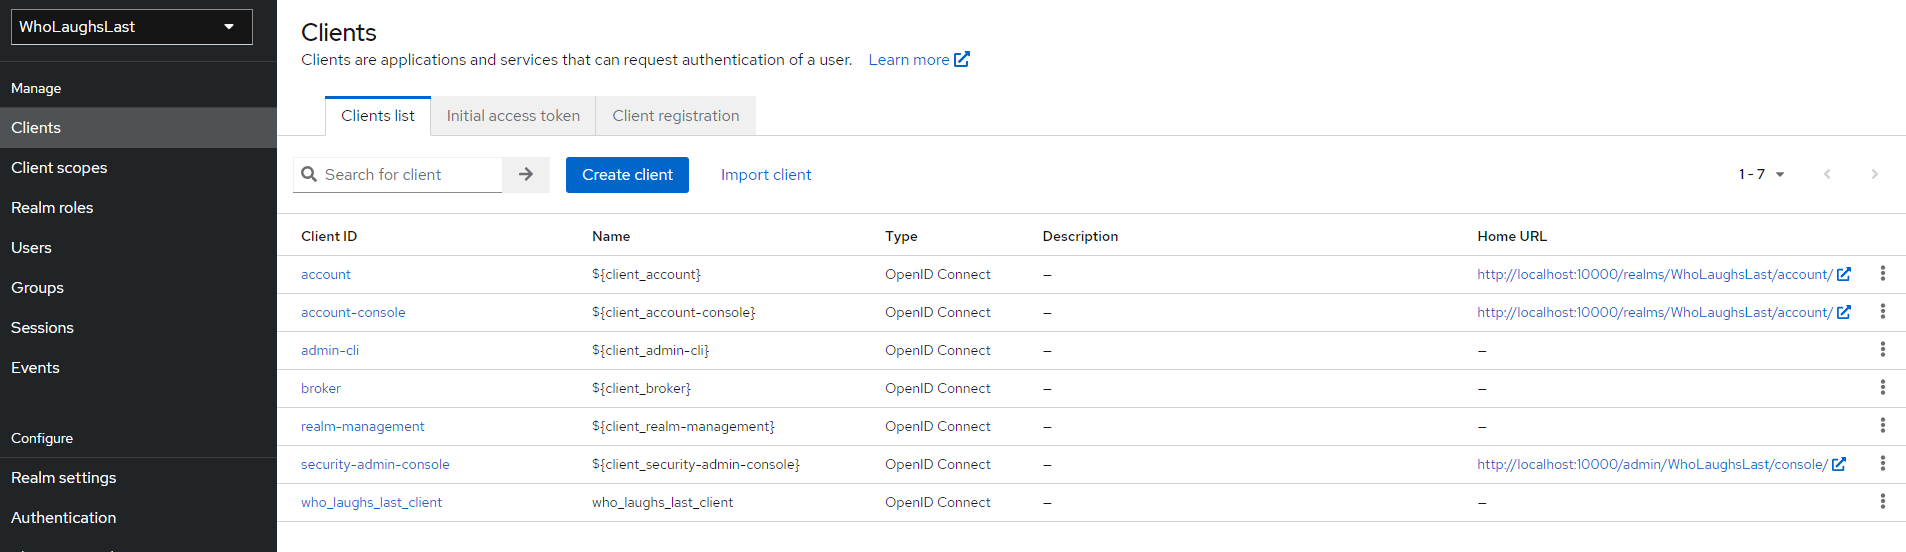
\includegraphics[scale=0.5]{keycloak-cients}
\end{figure}
Pár beállítást még kellett végezni a client-en. Először is megadtam a Valid redirect URL. Ez azt az elérési utat adja meg, ahova bejelentkezés után navigálni akarunk. Én 
a \textbf{http://localhost:3000/*} adtam meg, hiszen ezen a porton futott nekem a frontend alkalmazás, így a felhasználó bejelentkezés után bent volt az alkalmazásban. A keycloak
széles API-t kínál így ezt megismerve az backendemről authentikáció során ide küldtem a kéréseket. Azt is be lehet állítani hogy a mennyi idő után jár le az access token érvényessége, tehát utána majd újat kell kérni a szervertől. 

A végpontok biztonságossá tételéhez a \textbf{Spring Security}-t és az \textbf{OAuth2ResourceServer} dependency-ket használtam fel. A függőségeket leíró xml-eket beillesztettem a pom.xml fájlba, majd a Maven letöltötte őket, hogy majd használni tudjam. 

\begin{lstlisting}[language=XML, caption={A pom.xml fileban a függőségek},captionpos=b]
	<dependency>
		<groupId>org.springframework.boot</groupId>
		<artifactId>spring-boot-starter-oauth2-resource-server</artifactId>
		<version>3.1.5</version>
	</dependency>
	<dependency>
		<groupId>org.springframework.boot</groupId>
		<artifactId>spring-boot-starter-security</artifactId>
		<version>3.1.5</version>
	</dependency>
\end{lstlisting}

Miután a Spring Security bekerül az alkalmazásban, alapértelmezetten csinál egy SecurityFilterChain-t ami megköveteli hogy az összes API végpontnál
a hívónak authetntikálnia kell magát. Ezt a függvényt kell felülírni és úgy implementálni ahogyan azt mi szeretnénk. \textbf{@Bean} annotációval van ellátva,
így ezt a Spring kezeli és tudja hogy mikor kell használni. A kérések beérkeznek az alkalmazásunkba, akkor végighaladnak ezeken a filtereken amiket beállítunk. Miután talál 
egy olyan filtert ami a kéréshez illik: Például a "/board" végződésű végpontra jött kérés, akkor azt tudja hogy authentikálni kell, és a többi filtert már nem nézi meg, akár illik rá akár nem. 

\begin{figure}[h]
	\caption{SecurityFilterChain működése }
	\centering
	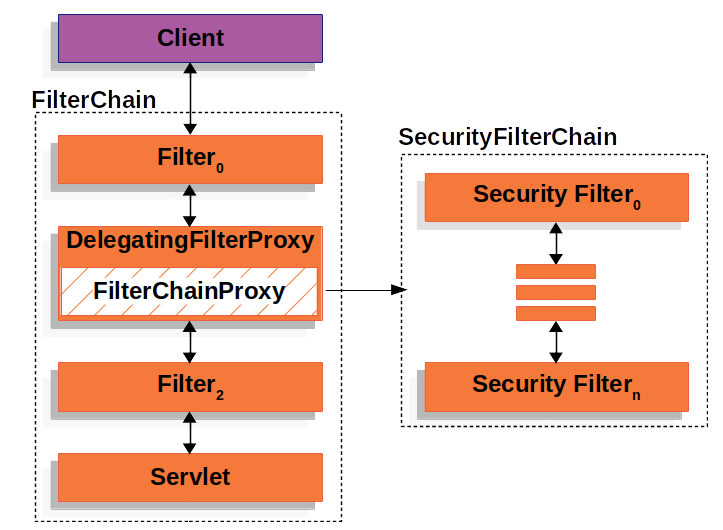
\includegraphics[scale=0.5]{filterchain}
\end{figure}

Úgy konfiguráltam fel a függvényt, hogy 3 végponton kívül mindent authetnikáljon: \textbf{/auth/createToken}, \textbf{/auth/refreshToken} ,\textbf{/subscribe}. Első kettőt végpontot azért nem kell authentikálni, mivel ide érkeznek azok a kérések amikor a felhasználó be akar jelentkezni, és kapja meg a szükséges token-eket amikre majd később szüksége lesz az authentikációnál.Ezek után a OAuth2 resource szervert kellett felkonfigurálni. Az application.yml file-ban írtam bele a különböző elérési utakat amikre a szervernek szüksége van hogy authentikálni tudja a jwt tokeneket. A keycloak-nál a \textbf{http://localhost:10000/realms/WhoLaughsLast/protocol/openid-connect/certs} elérési úton 
elérhető az adott client-hez tartozó authetnikációs adatok. A jwt tokeneket sütikben tárolva szállítottam a backend és frontend között. Ennek az egyik nagy előnye, hogy front-end részen a tokenek eltárolásával nem kell foglalkozni, így ha esetleg újratöltenénk az oldalt, az authentikációs tokeneink nem vesznek el. Ahhoz viszont hogy sütiket tudjunk küldeni, a CORS beállításnál engedélyezni kell, hogy engedélyezze a sütik küldését. 

\begin{lstlisting}[language=java,caption={SecurityConfig implementálása},captionpos=b]
@Configuration
@EnableWebSecurity
@EnableMethodSecurity
@RequiredArgsConstructor
public class SecurityConfig {
	
private final AuthService authService;

@Bean
public SecurityFilterChain securityFilterChain (HttpSecurity http)
													 throws Exception{
	System.out.println("Hallo");
	http
	.cors().and()
	.csrf()
	.disable()
	.authorizeHttpRequests(authorize -> authorize.
	requestMatchers("/auth/createToken","/auth/refreshToken")
	.permitAll()
	.anyRequest().authenticated()).oauth2ResourceServer()
	.jwt().and().
	bearerTokenResolver(authService::getAccesTokenFromCookie);
	
	http
	.sessionManagement()
	.sessionCreationPolicy(STATELESS);
	
	return http.build();
}
@Bean
CorsConfigurationSource corsConfigurationSource() {
	CorsConfiguration configuration = new CorsConfiguration();
	configuration.
	setAllowedOrigins(Arrays.asList("http://localhost:3000")); // Allow your frontend origin
	configuration.
	setAllowedMethods(Arrays.asList("GET", "POST", "PUT", "DELETE"));
	configuration.
	setAllowCredentials(true); // Allow credentials (cookies)
	configuration.addAllowedHeader("*");
		
	UrlBasedCorsConfigurationSource source = 
	new UrlBasedCorsConfigurationSource();
	source.registerCorsConfiguration("/**", configuration);
	return source;
	}
	
}
\end{lstlisting}

Ezek után implementáltam az authentikációs végpontot. Létrehoztam egy új Controllert aminek AuthController lett a neve,
hogy szeparáltan legyen a többi végponttól ami a játékhoz kell, az átláthatóság és a rendezettség érdekében.Az egyik végpont 
funkciója az hogy egy paraméterben kapott authorization code-ot elküldi a keycloak végpontjára amiért cserébe egy refresh tokent és egy access tokent kap.
Ezeket egy sütiben visszaadva juttatja el a frontendre. A másik végpont funkciója pedig az hogy egy paraméterben kapott refresh tokent beváltva új access tokent kapjon a frontend az authentikációhoz.  
\begin{lstlisting}[language=java,caption={Authentikációs végpont},captionpos=b]
@PostMapping("/createToken")
public void createToken(@RequestBody AuthTokenDTO authCode,
			HttpServletResponse httpServletResponse) throws Exception{
	TokenDTO tokenDTO =  authService.getTokens(authCode.getAuthCode());
	Cookie accesCookie =
	 new Cookie("access_token",tokenDTO.getAccess_token());
	Cookie refreshcookie =
	 new Cookie("refresh_token",tokenDTO.getRefresh_token());
	httpServletResponse.addCookie(accesCookie);
	httpServletResponse.addCookie(refreshcookie);
}

@PostMapping("/refreshToken")
public TokenDTO refreshAccesToken(@RequestBody RefreshTokenDTO refreshTokenDTO)
				 throws Exception{
	return authService.refreshAccesTokenWithRefreshToken(refreshTokenDTO
						.getRefresh_token());
}
\end{lstlisting}

\begin{figure}[h]
	\caption{Postman authentikációs token kérés}
	\centering
	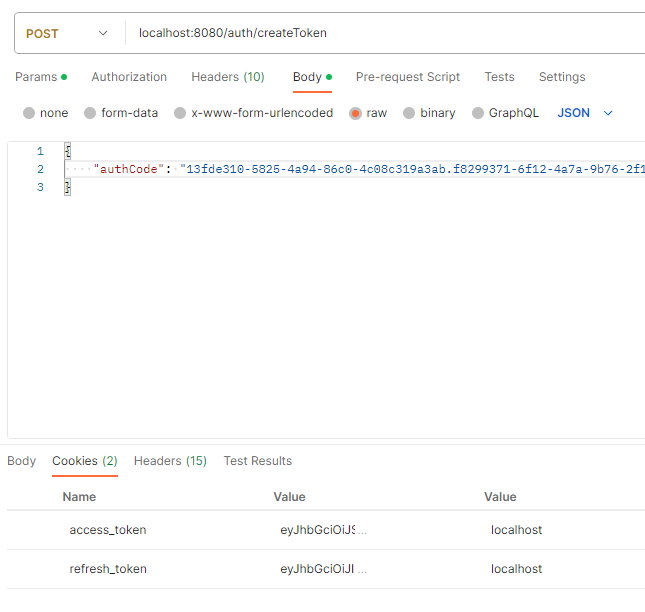
\includegraphics[scale=0.5]{getTokens}
\end{figure}
\newpage

\subsubsection{Frontend}
A frontenden az authentikáció egyik feladata az authorization code eljutattása a backend-re volt. Mivel használni akartam a keycloak által 
készített login paget, így az URL-ből kellett kivennem a code-nak az értékét. Mivel a megfelelő bejelentkezés után a keycloak átnavigál a frontend 
URL-jére, hiszen ezt beállítottuk az admin oldalon, így ezt az eseményt fel tudtam használni. Vue Routert használok a navigációra az alkalmazáson belül. A Vue Router 
sok hasznos funckióval rendelkezik, de ennél a problémánál a navigációs őröket (Navigation Guards) tudtam felhasználni. Itt meg tudok adni egy függvényt ami
mindig meghívódik azelőtt hogy navigáció történne az alkalmazáson belül. Tehát amikor megtörténik a navigáció a keycloak-os felületről az alkalmazásra, a függvény amit 
definiálok le fog futni. Paraméterként megkapom azt az elérési utat ahonnan navigáltak valamint azt is ahonnan navigáltak. Mivel ahhonnan navigálunk el ott jelenik meg az
authorization code, így ki tudom nyerni onnan. Egy újabb Pinia Store-t is definiáltam az authentikációhoz köthető függvények miatt a jó struktúráltság érdekében. Itt implementáltam egy api hivást, ami http kérés body-jában tárolja az authorization code-ot és küldi el a backend számára. Ha ez megtörténik a sütik tartalmazni fogják az access és refresh tokeneket, így elérem a többi végpontot ami a játék működéséhez kell a backenden. 
\begin{adjustwidth}{0cm}{0cm}
	\begin{minipage}{\textwidth}
		\begin{lstlisting}[style=javascriptStyle,caption={Authorization code kinyerése az elnavigált URL-ből}]
			router.beforeEach(async (to,from,next) => {
				const authStore = useAuthenticationStore();
				if(to.query.code) {
					console.log(to.query.code);
					await authStore.getAuthTokens({code: to.query.code});
					next(from.path);
				}
				else {
					next();
				}
			})
		\end{lstlisting}
	\end{minipage}
\end{adjustwidth}

\newpage

\subsection{Frontend}
A frontend készítésnél már volt egy kiinduló gitlab projektem, amit a külső konzulensem
biztosított számomra. Ez a projekt egy üres projekt volt, de a Vue.js keretrendszer, webpack
konfiguráció már importálva volt valamint, sok hasznos könyvtárat tartalmazott. Ahogy
korábban említettem, a Vue.js egy komponens orientált fejlesztés tesz lehetővé. Ezt használva
először azt terveztem meg hogy milyen komponensekből fog állni a megjelenítés.
Először a táblák megjelenítéséért felelős komponenst írtam meg. Ez listázza az összes
szerveren lévő táblát.
Következőleg az egy táblát reprezentáló komponenst implementáltam le. Itt látszódnak a tábla
fontosabb adatai, a különböző funkciójú gombok.
A Pinis Store implementálása következett. Itt definiáltam majd valósítottam meg az összes
aszinkron api hívást, hogy kényelmesen, az összes komponensből el tudjam érni őket. Itt
tárolom a táblákat, és egyéb megjelenítést segítő változókat.
Ezek után csináltam felugró ablakokat, ha egy játékost szeretnék egy táblához csatlakoztatni,
vagy egy új táblát szeretnénk létrehozni.
Mivel a backendem hibaüzenetet is adhat, hogyha inkonzisztens adatot küldök el, így annak
megjelenítésével is foglalkoznom kellett. Ha hiba adódik akkor, egy egyszerű piros ablak
jelenik meg az oldal tetején, amiben szerepel a hiba leírása. Ez az ablak 2,5 másodperc
elteltével eltűnik.



\newpage
\begin{thebibliography}{9}
	\bibitem{javaspring}
	Java Spring framework.
	
	\bibitem{vuejs}
	Vuejs framework.
	
	\bibitem{pinia}
	Pinia Store library.
	
	\bibitem{webpack}
	 Webpack is a static module bundler for modern JavaScript applications.
	 
	 \bibitem{axios}
	 Axios library
	 
	 \bibitem{lombok}
	 Lombok library
	 \bibitem{keycloak}
	 Keycloak library
	 \bibitem{konva}
	 Konva library
	 \bibitem{postman}
\end{thebibliography}

\end{document}